\documentclass[12pt,letterpaper,titlepage]{article}
\usepackage{solarized-light}
\usepackage{fontspec}
\defaultfontfeatures{Mapping=tex-text}
\usepackage{xunicode}
\usepackage{xltxtra}
\usepackage{amsmath}
\usepackage{pdfpages}
\usepackage{amsfonts}
\usepackage{amssymb}
\setcounter{secnumdepth}{0}
\usepackage{nameref}
\usepackage{enumitem}
\usepackage{environ}
\usepackage{pgfplots}
\usepackage{karnaugh-map}

\setmainfont{Times New Roman}
\showboxdepth=\maxdimen
\showboxbreadth=\maxdimen


\usepackage{paracol}
\usepackage{wrapfig}
\globalcounter{table}
\globalcounter{figure}
\usepackage{graphicx}
\usepackage[left=1in,right=1in,top=1in,bottom=1in]{geometry}
\graphicspath{{img/}}

\author{Jacob Abel}
\title{	Homework 3
	\\\large ECE3544 CRN:82989
}

\setlength{\parskip}{0.25em}

\begin{document}
\maketitle
\begin{raggedright}
\paragraph{Note: }

For problems 2, 3, 4, and 6 you should create a test bench to validate your modules and show correct operation for all input combinations of 0's and 1's (don't worry about combinations with x's and z's). Your PDF solution should include waveforms displaying correct operation of each module.

\paragraph{Problem 1: }
Explain why the code fragment below will execute forever. Provide a working alternative.

\begin{lstlisting}
reg [1:0] loop1;
for (loop1 = 0; loop1 <= 4; loop1 = loop1 + 1)
begin
    some statements;
end
\end{lstlisting}

The register is 2-bits wide and therefore has a max unsigned value of 3. This means every possible value is less than 4 and the loop will run even after it overflows back to 0. The below is a functional statement.

\begin{lstlisting}
reg [2:0] loop1;
for (loop1 = 0; loop1 <= 4; loop1 = loop1 + 1)
begin
    some statements;
end
\end{lstlisting}

\clearpage

\paragraph{Problem 2: }
A 7-segment display is often used to display decimal numbers. Shown below is one such unit with the segments labelled a-g (we will ignore the decimal point p). Each of the segment outputs is lit on when a '0' is applied to it and is off when a'1' is applied to it. Create a data-flow model using only continuous assignments of a device that accepts a four-bit binary number representing decimal numbers 0-15, and drives the appropriate segments of a 7-segment display to display the number in hex. 

Please note: the number 6 should have all segments except "b" on, and the number 9 should have all segments except "e" on. For hexadecimal numbers A, C, E, and F, the display should show upper case, while for B and D, it should show lower case (i.e., the number B should have all segments but "a" and "b" on, while the number D should have all segments but "a" and "f" on).
\begin{center}
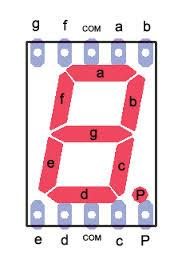
\includegraphics[width=\textwidth, height=9\baselineskip, keepaspectratio=true]{hw3q2}
\end{center}

\begin{lstlisting}
// Insert your header here, using the starter files from project
// 1a and the documentation lecture as a guide.

module sevensegdecoder_assign(d3, d2, d1, d0, a_n, b_n, c_n, d_n, 
e_n, f_n, g_n);
input d3, d2, d1, d0; // active high inputs
output a_n, b_n, c_n, d_n, e_n, f_n, g_n; // active low outputs
//
// I N S E R T Y O U R C O D E H E R E
// E N D I N S E R T
endmodule
\end{lstlisting}

Incomplete

\clearpage

\paragraph{Problem 3: }
Repeat problem 2 using a procedural model using only an always block with a case or if statement. The module declaration is given below.

\begin{lstlisting}
module sevensegdecoder_always(d3, d2, d1, d0, a_n, b_n, c_n, d_n, 
e_n, f_n, g_n);
input d3, d2, d1, d0; // active high inputs
output a_n, b_n, c_n, d_n, e_n, f_n, g_n; // active low outputs
\end{lstlisting}

Incomplete

\clearpage

\paragraph{Problem 4: }
Create a procedural model for a combinational circuit that counts the number of ones in a byte.The input to the circuit should be an 8-bit array named byte\_in, with bit 7 as the leftmost bit and bit 0 as the rightmost bit. The output of the circuit should be a four-bit array named ones, with bit 3 as the leftmost bit and bit 0 as the rightmost bit.

Incomplete

\clearpage

\paragraph{Problem 5: }
Implement the function $F(a, b, c, d) = \Sigma(0, 1, 2, 5, 7, 9, 11, 14, 15)$ using Shannon’s expansion theorem and a 2-to-1 mux. For the expansion, use variable a as the variable to select between $F(0, b, c, d)$ (i.e., the function with $a=0$) and $F(1, b, c, d)$ (i.e., the function with a=1), and then use a as the select line for the 2-to-1 mux. Your solution should be a schematic showing the mux and the functions used as data inputs to the mux.

\begin{center}
\begin{karnaugh-map}[4][4][1][$cd$][$ab$]
  \minterms{0,1,2,5,7,9,11,14,15}
  \autoterms[0]
\end{karnaugh-map}

$F(a, b, c, d) = \Sigma(0, 1, 2, 5, 7, 9, 11, 14, 15)$

$F(a, b, c, d) = \overline{a}\cdot G(b, c, d) + a\cdot H(b, c, d)$

\end{center}
\begin{paracol}{2}
\begin{center}
\begin{karnaugh-map}[4][2][1][$bc$][$a$]
  \minterms{0,1,2,5,7}
  \autoterms[0]
\end{karnaugh-map}

$G(a, b, c) = \Sigma(0, 1, 2, 5, 7)$
\end{center}
\switchcolumn
\begin{center}
\begin{karnaugh-map}[4][2][1][$bc$][$a$]
  \minterms{2,3,5,7}
  \autoterms[0]
\end{karnaugh-map}

$H(a, b, c) = \Sigma(2, 3, 5, 7)$
\end{center}
\end{paracol}

\begin{center}
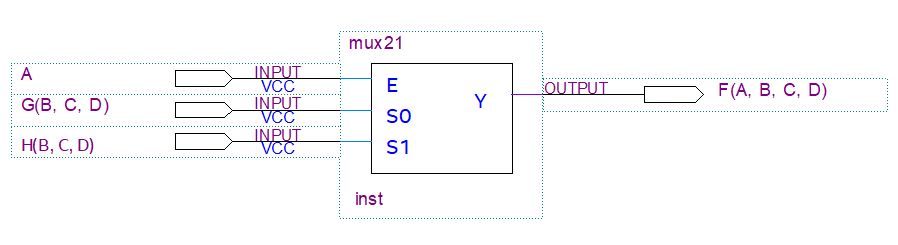
\includegraphics[width=\textwidth, height=9\baselineskip, keepaspectratio=true]{hw3q5}
\end{center}

\clearpage

\paragraph{Problem 6: }
Implement your solution for problem 5 in Verilog and verify its operation. Create a behavioural module for a 2-to-1 mux named mux21, then create a module named homework3\_problem6 that instantiates your mux21 module. The homework3\_problem6 module should have input ports a, b, c and d, and output port F. You should then create a test bench to validate your module and show correct operation for all input combinations.

\begin{center}
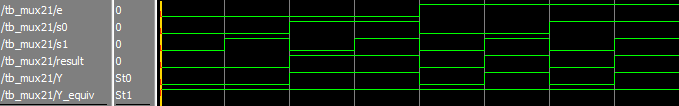
\includegraphics[width=\textwidth, height=9\baselineskip, keepaspectratio=true]{hw3q6a}
mux21 Simulation Results (Y\_equiv demonstrates equivalence to expected result (result))
\end{center}

\end{raggedright}
\end{document}
